%%%%%%%%%%%%%%%%%%%%%%%%%%%%%%%%%%%%%%%%%
% NIWeek 2014 Poster by T. Reveyrand
% www.microwave.fr
% http://www.microwave.fr/LaTeX.html
% ---------------------------------------
%
% Original template created by:
% Brian Amberg (baposter@brian-amberg.de)
%
% This template has been downloaded from:
% http://www.LaTeXTemplates.com
%
% License:
% CC BY-NC-SA 3.0 (http://creativecommons.org/licenses/by-nc-sa/3.0/)
%
%%%%%%%%%%%%%%%%%%%%%%%%%%%%%%%%%%%%%%%%%

%----------------------------------------------------------------------------------------
%   PACKAGES AND OTHER DOCUMENT CONFIGURATIONS
%----------------------------------------------------------------------------------------

\documentclass[a0paper,portrait]{baposter}

\usepackage[font=small,labelfont=bf]{caption} % Required for specifying captions to tables and figures
\usepackage{booktabs} % Horizontal rules in tables
\usepackage{relsize} % Used for making text smaller in some places
\usepackage{amsmath,amsfonts,amssymb,amsthm} % Math packages
\usepackage{eqparbox}
\usepackage{textcomp}
\usepackage{caption}
\usepackage{subcaption}
\usepackage{graphicx}
\usepackage{listings}
\usepackage{enumitem}
\usepackage{pgf}
\usepackage{tikz}
\usetikzlibrary{positioning}
\usepackage[utf8]{inputenc}
\usetikzlibrary{arrows,automata}
\usetikzlibrary{positioning}
\usepackage{hyperref}


\graphicspath{{figures/}} % Directory in which figures are stored

 \definecolor{bordercol}{RGB}{40,40,40} % Border color of content boxes
 \definecolor{headercol1}{RGB}{186,215,230} % Background color for the header in the content boxes (left side)
 \definecolor{headercol2}{RGB}{120,120,120} % Background color for the header in the content boxes (right side)
 \definecolor{headerfontcol}{RGB}{0,0,0} % Text color for the header text in the content boxes
 \definecolor{boxcolor}{RGB}{210,235,250} % Background color for the content in the content boxes


\tikzset{
    state/.style={
           rectangle,
           rounded corners,
           draw=black, very thick,
           minimum height=2em,
           inner sep=2pt,
           text centered,
           },
}

\begin{document}

\setlength{\fboxsep}{0pt}

\background{ % Set the background to an image (background.pdf)
\begin{tikzpicture}[remember picture,overlay]
\draw (current page.north west)+(-2em,2em) node[anchor=north west]
{
\includegraphics[height=1.1\textheight]{background}};
\end{tikzpicture}
}

\begin{poster}{
grid=false,
columns=4,
borderColor=bordercol, % Border color of content boxes
headerColorOne=headercol1, % Background color for the header in the content boxes (left side)
headerColorTwo=headercol2, % Background color for the header in the content boxes (right side)
headerFontColor=headerfontcol, % Text color for the header text in the content boxes
boxColorOne=boxcolor, % Background color for the content in the content boxes
headershape=roundedright, % Specify the rounded corner in the content box headers
headerfont=\Large\sf\bf, % Font modifiers for the text in the content box headers
textborder=rectangle,
background=none,
headerborder=open, % Change to closed for a line under the content box headers
boxshade=plain
}
{
\includegraphics[width=3cm]{BiATA2019.png}}
%
%----------------------------------------------------------------------------------------
%   TITLE AND AUTHOR NAME
%----------------------------------------------------------------------------------------
%
{ \bf  \huge {Improved Architecture of Artificial Neural Network for Secondary Structure Analysis} }  % Poster title
{\vspace{0.3em} \smaller \textbf{Polina Lunina$^1$}, Semyon Grigorev$^1$ \\  % Author names
\smaller \it $^1${Saint Petersburg State University, JetBrains Reserach, St. Petersburg, Russia } \\ % Author email addresses
\smaller  {\textbf{E-mail:} lunina\_polina@mail.ru, semyon.grigorev@jetbrains.com}}
{
\includegraphics[width=3cm]{SPbGU_Logo.png}} % University/lab logo


%----------------------------------------------------------------------------------------
%   INTRODUCTION
%----------------------------------------------------------------------------------------
\headerbox {Motivation}{name=introduction,column=0,row=0, span=2}{

Existing solution for secondary structure analysis~\cite{grigorevcomposition}:\\
%\begin{enumerate}
  %\item sequance $\to$ parser $\to$ boolean matrix (\textbf{})
  %\item boolean matrix $\to$ int vector (\textbf{problems with size and data locality})
  %\item int vector $\to$ dence neural network
%\end{enumerate}
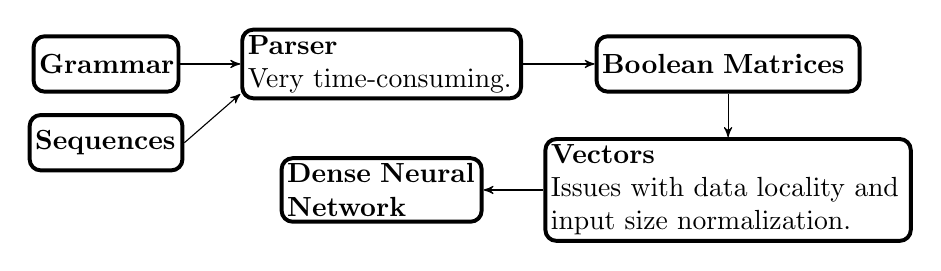
\begin{tikzpicture}[->,>=stealth']

  \node[state,
        line width=0.5mm,
        %left of = parser,
        align=left,
        text width = 1.7cm] (grm)
   {
    \textbf{Grammar}
   };

  \node[state,
        line width=0.5mm,
        below of=grm,
        node distance=1cm,
        align = left,
        text width = 1.8cm] (sqs)
   {
   \textbf{Sequences}
   };

\node[state,
      line width=0.5mm,
      align = left,
      right of = grm,
      node distance=3.5cm,
      text width = 3.4cm](parser)
{
\textbf{Parser} \\ Very time-consuming.
};

\node[state,
      line width=0.5mm,
      right of=parser,
      node distance=4.4cm,
      align = left,
      text width = 3.2cm] (mtrx)
{
  \textbf{Boolean Matrices}
};

\node[state,
      line width=0.5mm,
      below of=mtrx,
      node distance=1.6cm,
      align = left,
      text width = 4.5cm](vector)
{
\textbf{Vectors}\\
Issues with data locality and input size normalization.
};

\node[state,
      line width=0.5mm,
      %below of = parser,
      left of = vector  ,
      align = left,
      node distance=4.4cm,
      text width = 2.4cm](NN)
{
\textbf{Dense Neural Network}
};

\path (grm.east) edge (parser)
 (sqs.east) edge (parser.192)
 (parser) edge (mtrx)
 (mtrx) edge (vector)
 (vector) edge (NN);
 %(NN.-10.5) edge [-,dashed,black] (NN_info)

\end{tikzpicture}

Questions:
\begin{itemize}
  \item \textbf{Is it possible to move parsing to network training step?}
  \item \textbf{Is it possible to use convolutional neural networks for \\ parsing result processing?}
\end{itemize}

}


\headerbox {Parsing Elimination}{name=pElim, column=0, row=0, span=2, below=introduction}{

 We solve this problem by using two-staged learning.
 \begin{enumerate}
   \item Train a network which takes parsed data as an input (\textbf{base model}).
   \item Extend the~trained network with a number of layers that convert the~nucleotide sequence into a parsing result (\textbf{extended model}).
 \end{enumerate}
    %This way we create a network which can handle sequences, not parsing result.
    \textbf{Parsing is required only for network training.}
}

\headerbox {Results: tRNA Classification}{name=results, column=2, row=0, span=2}{
\begin{itemize}
  \item 2 classes: eukaryotes and prokaryotes (EP).
  \item 4 classes: archaea, bacteria, fungi and plants (ABFP).
\end{itemize}
\begin{center}
\small
\begin{tabular}{|l||l|l||l|l|}
\hline
Classifier                                                               & \multicolumn{2}{c||}{EP}               & \multicolumn{2}{c|}{ABFP}           \\ \hline \hline
Approach   & Vectors  & Images   & Vectors      & Images     \\ \hline
\begin{tabular}[c]{@{}l@{}}Base model\\ accuracy\end{tabular}            & 94.1\%             & 96.2\%           & 86.7\%            & 93.3\%          \\ \hline
\begin{tabular}[c]{@{}l@{}}Extended model \\ accuracy\end{tabular}       & 97.5\%             & 97.8\%           & 96.2\%            & 95.7\%          \\ \hline
\begin{tabular}[c]{@{}l@{}}Total samples\\ (train:valid:test)\end{tabular} & \multicolumn{2}{c||}{20000:5000:10000} & \multicolumn{2}{c|}{8000:1000:3000} \\ \hline
\end{tabular}
\end{center}
Sequences from open databases~\cite{trnadb1, trnadb2}.

}

\headerbox {Convolutional Networks}{name=dFormat, column=2, row=0, span=2, below=results}{

\begin{minipage}[t]{7.1cm}
  \vspace{-2.8cm}
 Matrices can be treated as bitmaps.
\begin{itemize}
  \item Images can be easily resized.
  \item Data locality is preserved.
  \item \textbf{We can use convolutional networks.}
\end{itemize}
\end{minipage}
~
\begin{minipage}[b]{3cm}
  \fbox{
\includegraphics[width=2.8cm]{figures/mt1.png}}
\end{minipage}
}

\headerbox{Solution Overview}{name=solution,span=4,column=0,row=1,below=pElim}{

\begin{tikzpicture}[->,>=stealth']

  \node[state,
        line width=0.5mm,
        %above left=2.25cm and -1.5cm of NN,
        align=left,
        text width = 1.8cm] (grm)
   {
    \textbf{Grammar}
   };

  \node[state,
        line width=0.5mm,
        below of=grm,
        node distance=1cm,
        align = left,
        text width = 1.8cm] (sqs)
   {
   \textbf{Sequences}
   };


\node[state,
      line width=0.5mm,
      align = left,
      below right = -0.7 and 0.5 of grm,
      node distance = 5cm,
      text width = 6cm](parser)
{
\textbf{Parser}\\
Extracts secondary structure features described by a~grammar.\\
Matrix-based parsing algorithm~\cite{gsv}.
};

\node[state,
      line width=0.5mm,
      right of=parser,
      node distance=6.3cm,
      align = left,
      text width = 5cm] (mtrx)
{
  \textbf{Matrices}\\
$w$ -- sequence,  $N$ -- nonterminal. \\ $M_N [i,j] = 1$, iff $w[i,j-1]$ is derivable from $N$.
};

\node[state,
      line width=0.5mm,
      right of=mtrx,
      node distance=6cm,
      align = left,
      text width = 5.5cm](vector)
{
\textbf{Vectors}\\
%\begin{enumerate}
  Drop out the~bottom left triangle. \\
  Vectorize matrix row by row. \\
  Length normalization is requried. \\
%\end{enumerate}
};

\node[state,
      line width=0.5mm,
      below right = 1 and -0.7 of mtrx,
      node distance=3cm,
      align = left,
      text width = 3.4cm](image)
{
\textbf{Images}\\
\vspace{-0.2cm}
\begin{center}
\fbox{
\includegraphics[width=3cm]{figures/mt1.png}}
\end{center}
};

\node[state,
      line width=0.5mm,
      below of=parser,
      node distance=5.8cm,
      align = left,
      text width = 11.6cm](NN)
{
\textbf{Neural Networks}\\
 %\vspace{0.2cm}
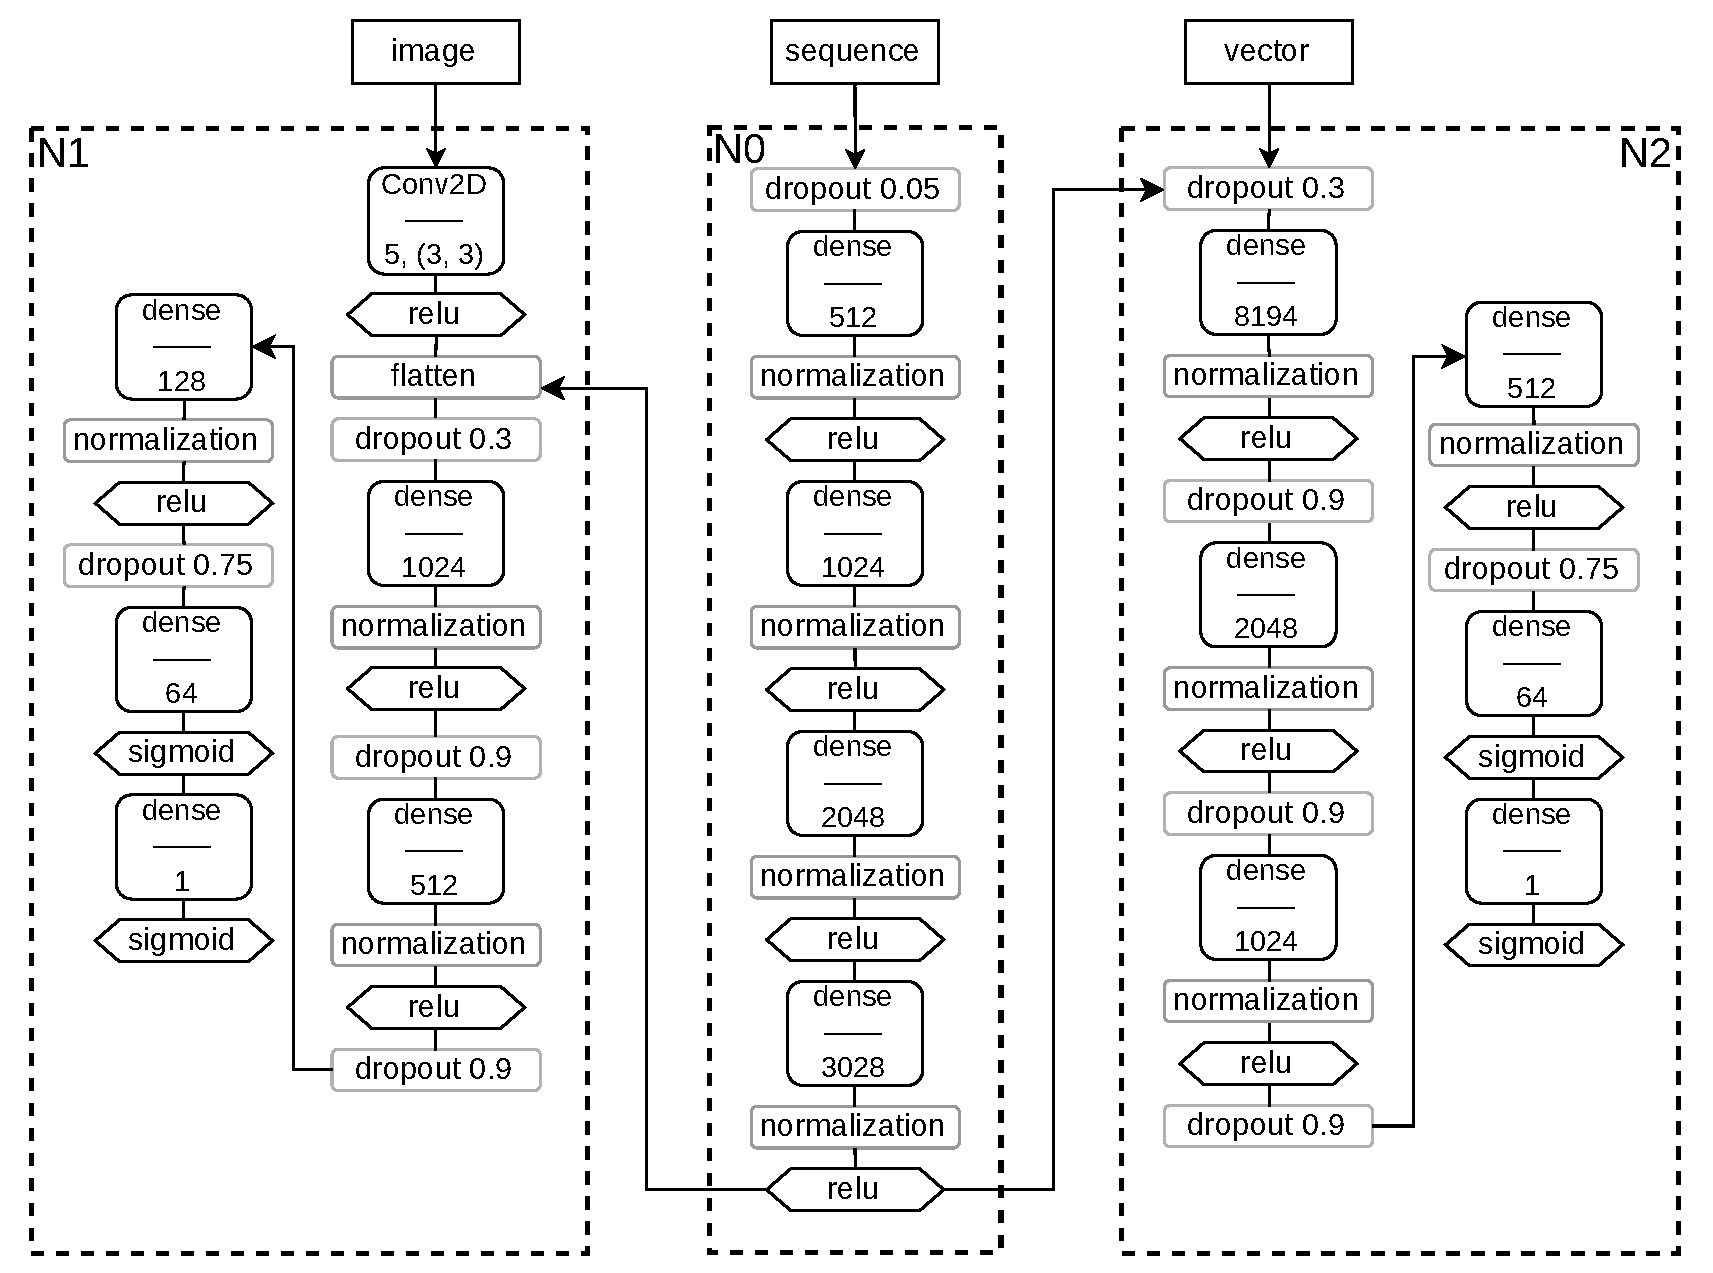
\includegraphics[width=11.4cm]{figures/nn_arch.pdf}

};


\node[state,
      line width=0.5mm,
      below of = image,
      node distance = 4 cm,
      align = left,
      text width = 7cm](NN_info)
{
\textbf{Neural Networks}\\
\textbf{\texttt{N1}} -- images classification.\\
\textbf{\texttt{N2}} -- vectorized data classification.\\
\textbf{\texttt{N0}} -- the~extension block which converts the~nucleotide sequence into a~set of features for \textbf{\texttt{N1}} or \textbf{\texttt{N2}}.


};

\node[
      line width=0.5mm,
      below right = -1.3 and 1.1 of NN_info,
      align = left,
      text width = 2.7cm](qr)
{

\includegraphics[width=2.5cm]{figures/qr-research-jetbra.pdf}
};



\path (grm.east) edge (parser)
 (sqs.east) edge (parser)
 (parser) edge (mtrx)
 (mtrx) edge (vector)
 (mtrx) edge (image)
 (vector) edge [bend left] (NN_info)
 (NN.-17) edge [-,dashed,black] (NN_info)
 (image) edge (NN_info);
\draw (sqs.south) -- (0.0,-1.6) --(11.5,-1.6) -- (NN_info.157.7);

\end{tikzpicture}
}


\headerbox {Future Research}
{name=app1,column=0,span=2, below=solution}
{
\begin{itemize}
\item 16s rRNA processing and chimeric sequences filtration.
\item Proteomic sequences processing, proteins functions prediction.
\item Generative networks for sequences secondary structure prediction.
\end{itemize}

}

%----------------------------------------------------------------------------------------
%   REFERENCES
%----------------------------------------------------------------------------------------

\headerbox {References}
{name=app2,column=2,span=2, below=solution}
{
%\smaller % Reduce the font size in this block
\renewcommand{\section}[2]{\vskip 0.05em} % Get rid of the default "References" section title
%\nocite{*} % Insert publications even if they are not cited in the poster
\small
\bibliographystyle{unsrt}
%\bibliographystyle{IEEEtran}
\bibliography{biblio} % Use biblio.bib as the bibliography file
\vspace{0.34cm}
}


\headerbox {Acknowledgments}{name=ack,column=0,span=2,below=app1}{
the~research was supported by the~Russian Science Foundation grant \\ 18-11-00100 and a grant from JetBrains Research.
}

\headerbox {Information}{name=info,column=0,span=2,below=ack}{
Trained models and other materials are published at GitHub:\\
\url{https://github.com/LuninaPolina/SecondaryStructureAnalyzer}.
}

\end{poster}

\end{document}
